%%%%%%%%%%%%%%%%%%%%%%%%%%%%%%%%%%%%%%%%%%%%%%%%%%%%%%%%%%%%%%%%%%%%
%% I, the copyright holder of this work, release this work into the
%% public domain. This applies worldwide. In some countries this may
%% not be legally possible; if so: I grant anyone the right to use
%% this work for any purpose, without any conditions, unless such
%% conditions are required by law.
%%%%%%%%%%%%%%%%%%%%%%%%%%%%%%%%%%%%%%%%%%%%%%%%%%%%%%%%%%%%%%%%%%%%

% This theme was based on fibeamer theme 
% If you found any bugs please contact @karlosos
% This repository is hosted on github https://github.com/karlosos/zut-fibeamer/

\documentclass{beamer}
\usetheme[faculty=wi]{fibeamer}
\usepackage[utf8]{inputenc}
\usepackage[
  main=polish,
  polish
]{babel}

\title{Aula 10  - Banco de dados}
\subtitle{Tópicos especiais em Sistemas}
\author{Prof. Juliana Costa Silva - juliana.silva@up.edu.br}

\usepackage{ragged2e}  % `\justifying` text
\usepackage{booktabs}  % Tables
\usepackage{tabularx}
\usepackage{tikz}      % Diagrams
\usetikzlibrary{calc, shapes, backgrounds}
\usepackage{amsmath, amssymb}
\usepackage{url}       % `\url`s
\usepackage{listings}  % Code listings
\frenchspacing
\begin{document}

%------------------------------------------------------------------------
  \frame[c]{\maketitle}
      \begin{frame}<beamer>
      \frametitle{O que veremos hoje}
      \tableofcontents
    \end{frame}
%------------------------------------------------------------------------
    \section{Revendo...}
    \begin{frame}{Revendo...}{O que já aprendemos?}
      
      \begin{itemize}
            \item Criamos um projeto node;
            \item Organizamos os arquivos de configuração na pasta config;
            \item Organizamos os controladores na pasta controllers;
            \item Enviamos dados em formato JSON
       \end{itemize}
     \end{frame}
     %------------------------------------------------------------------------
\begin{frame}[label=proof]{Para começar...}
	\begin{itemize}
	\item Restaure o projeto da aula anterior;
	\item Este sistema deve ter a estrutura de pastas e arquivos apresentada abaixo:
	\end{itemize}
	\begin{center}
	    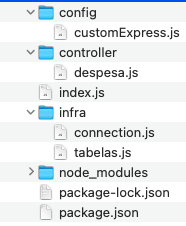
\includegraphics[width=45mm]{resources/aula10_1.png} \\ \tiny{\textbf{Estrutura do projeto}}
	\end{center}
    \end{frame}
%------------------------------------------------------------------------
    \begin{frame}[label=lists]{Models}
      \begin{columns}[onlytextwidth]
        \column{.5\textwidth}
          \begin{itemize}
            \item Vamos trabalhar com models, para a isolar as regras de inserção, deleção, edição e consulta;
            \item Cria uma pasta \textbf{model} na raiz do projeto. Nessa pasta crie o arquivo movimento.js;
          \end{itemize}
        \column{.5\textwidth}
            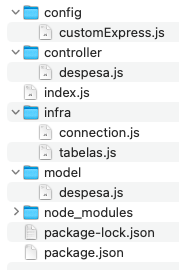
\includegraphics[width=40mm]{aulas/resources/aula10_2.png} \\
            \tiny{\textbf{Estrutura do projeto}}
      \end{columns}
    \end{frame}

%------------------------------------------------------------------------
\section{Infraestrutura}
    \begin{frame}[label=lists]{Infraestrutura}
    \begin{exampleblock}{Pasta de infraestrutura}
        	\begin{itemize}
	\item Essa pasta será responsável por arquivos de infraestrutura;
	\item Tudo o que é necessário para a aplicação funcionar além das regras de negócio;
	\item Crie uma pasta \alert{infra} e dentro dela o arquivo \textbf{conncetion.js}.
        	\end{itemize}
        	\tiny{\cite{nodejs2022api, moziladev2022js}}
      \end{exampleblock}
    \end{frame}
%------------------------------------------------------------------------
\section{INSERT}
    \begin{frame}[label=lists]{Inserção}

% \begin{columns}[onlytextwidth]
%        \column{.5\textwidth}
         Para realizar a inserção precisamos receber os dados que serão inseridos, chamaremos esse objeto de \alert{movimento};
         \begin{itemize}
         \item Crie a classe Moviemnto;
         \item Importe o módulo \textbf{connection.js};
         \item Implemente o método adiciona, que fará o insert no banco de dados;
         \end{itemize}
%        \column{.5\textwidth}
	            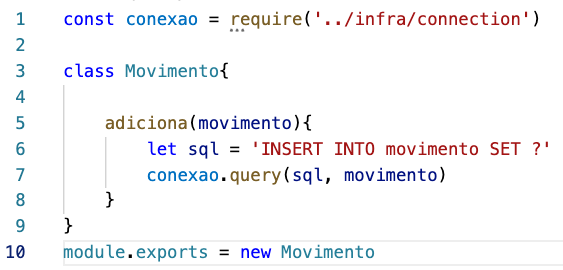
\includegraphics[width=80mm]{aulas/resources/aula10_3.png}\\
            \tiny{\textbf{Fonte:} O autor}
%      \end{columns}
    \end{frame}

 %------------------------------------------------------------------------
    \begin{frame}[label=lists]{Tratamento de exceção}
    Note que é necessário verificar se a inserção foi executada com sucesso!
   \begin{itemize}
       \item Se a conexão não der certo a aplicação não deveria funcionar;
       \item Para isso acrescente o tratamento de erro com um \alert{if, else} na execução do INSERT;
    \end{itemize}
    \begin{center}
    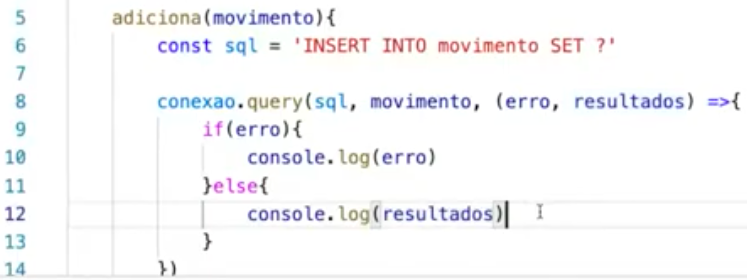
\includegraphics[width=80mm]{aulas/resources/aula10_4.png}\\
            \tiny{Método adiciona\textbf{Fonte:} O autor}
      \end{center}
    \end{frame}

%------------------------------------------------------------------------
\section{Referências}
    \begin{frame}{Referências}%[allowframebreaks]
\frametitle{Referências}
\small
\begin{center}
\tiny
\bibliographystyle{apalike}
\bibliography{./ref_aula}
\end{center}
\end{frame}
  
\end{document}
